\section{Some Evidence}

\paragraph{Belief heterogeneity and stock market turnover.}  
A salient feature of models with heterogeneous beliefs is their predictions regarding stock-market turnover. In this section, we use our estimates to construct a time series of belief disagreements and present its correlation with a measure of stock turnover. 

Recall that the expectation of analyst of aggregate earnings growth is given by $\mathbb{E}_i[\Delta e_{t+1}] = \theta_i \Delta e_t$. 
We use the following \textit{disagreement index} $DI_t$,:
\begin{equation}
    DI_t = \underbrace{\overline{\sigma}[\theta_i] \times | \Delta e_t | }_{\overline{\sigma}[\mathbb{E}_i[\Delta e_{t+1}] ] }.
\end{equation}
% \begin{figure}[t!]
%     \caption{Kernel estimate of cross-sectional distribution of the different parameters}
%     \begin{center}
%             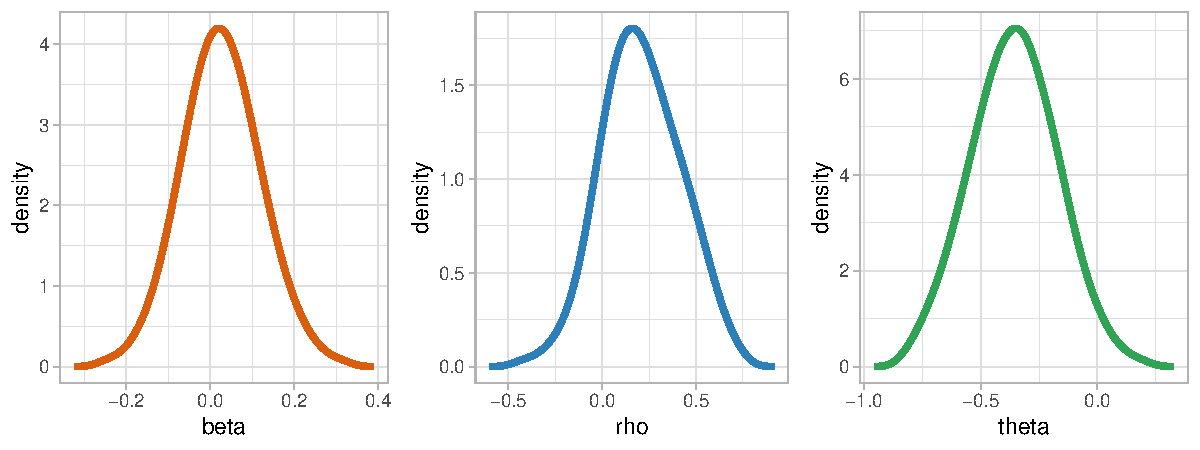
\includegraphics[width=1.0\textwidth]{figures/kernel_densities.pdf}
%     \end{center}
%     \caption*{  \scriptsize Note: Posterior mean of the kernel density for the cross-section of $\theta_i$ (left panel), $\rho_i$ (middle panel), and $\theta_i$ (right panel).\par} 
%     \vspace{0.0cm}
%     \label{fig: kernel_estimates}
% \end{figure}
The disagreement index (DI) has two components: First, the cross-sectional dispersion in $\theta_i$. Second, the absolute value of current aggregate earnings growth, $|\Delta e_t|$. If all analysts were to agree on the persistence of aggregate earnings growth, such that $\overline{\sigma}[\theta_i] = 0$, then the DI would equal zero. In turn, given that $\Delta e_t$ has already been demeaned, $|\Delta e_t|$ captures the distance of aggregate earnings growth to the mean. 
Also, there is no disagreement if aggregate earnings growth is at its average value, $|\Delta e_t| = 0$. Thus, the DI increases with the deviations from the mean of aggregate earnings and more so with the underlying disagreement about the reversal speed.  

The left panel of Figure \ref{fig: DI_turnover_time_series} shows the time series of DI. Disagreement is low during expansions, but spikes in recessions, the periods where earnings growth deviates most from the mean.

We relate the value-weighted stock-market turnover with the DI.% \footnote{For a discussion of turnover as a measure of trading volume and its connection with standard portfolio theory, see \citet{lo2010stock}.} 
\footnote{We measure the stock turnover - shares traded divided by shares outstanding---for individual securities on the New York and American Stock Exchanges from January 1977  to December 2021. We measure turnover at the quarterly frequency and compute an aggregate turnover measure using a value-weighted average (similar results are obtained by using an equal-weight measure).}
The right panel of Figure \ref{fig: DI_turnover_time_series} shows that turnover increased significantly over time. Moreover, it shows an important countercyclical behavior.
% potentially reflecting an increase in market participation, 
%, as shown by the difference between the turnover and its HP-filtered trend.

\begin{figure}[t!]
    \caption{Time series of the disagreement index and stock market turnover}
    \begin{center}
            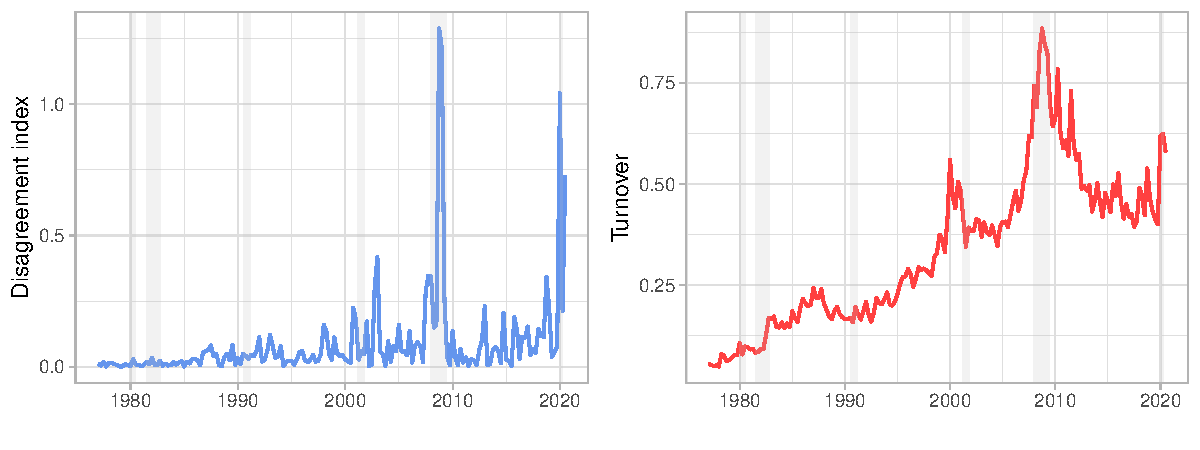
\includegraphics[width=1.0\textwidth]{figures/DI_turnover_time_series.pdf}
    \end{center}
    \caption*{  \scriptsize Note: Left panel shows the time series of the disagreement index and the right panel shows the time series of stock market turnover. The smooth line in the right panel is the HP-filter trend of turnover. The vertical bars represent NBER recessions.\par} 
    \vspace{0.0cm}
    \label{fig: DI_turnover_time_series}
\end{figure}

Table \ref{tab:reg_turnover_DI} shows the result of a time-series regression of turnover against the DI. In line with the visual inspection of Figure \ref{fig: DI_turnover_time_series}, the disagreement DI features outliers during recessions. We thus exclude observations where the DI is below the $2.5\%$ percentile or above the $97.5\%$ percentile. 
Column (1) shows a strong statistically significant correlation between DI and turnover.
% SB: ---we compute Newey-West standard-errors with four lags. To bottom of table!
If the disagreement index increases from the $25\%$ percentile value to its $75\%$ percentile value, turnover increases
% by $8.0$ percentage points, an increase of 
by almost $30\%$. 
Column (2) shows that turnover responds particularly strongly to the DI during downturns. 
We add an interaction of the DI with a dummy for NBER recessions and find that the coefficient is positive and statistically significant; its magnitude is economically large, and the response of turnover to the DI is $70\%$ larger in recessions. 
Column (3) tests for a nonlinear relationship: we introduce a quadratic term, again excluding outliers. The quadratic term is non significant. %, consistent with a linear relationship---see also Figure \ref{fig: DI_turnover_scatter}, which shows this sample's scatterplot of turnover and the disagreement index.
Column (4) performs the same non-linear regression but includes outliers. In this case, the quadratic term becomes statistically significant, again indicating that the outliers also capture increased disagreement during downturns. 
% The magnitude of the linear terms in the regressions is similar in all cases. 

In conclusion, the DI is strongly correlated with turnover, but more so in crises. Recall that above we show that extrapolative beliefs are consistent with this prediction.

\begin{table}[t!]
    	\centering
    	\caption{Regression of turnover on disagreement index}
 	\begin{tabular}{lcccc}
   \tabularnewline \midrule \midrule
   Dependent Variable: & \multicolumn{4}{c}{$turnover$}\\
   Model:         & (1)            & (2)            & (3) & (4)\\  
   \midrule
   \emph{Variables}\\
   (Intercept)    & 0.258$^{***}$ & 0.262$^{***}$ & 0.242$^{***}$ & 0.255$^{***}$\\   
                  & (0.034)      & (0.042)       & (0.044)       & (0.037)\\   
   $DI$             & 1.239$^{***}$  & 1.066$^{**}$  & 1.798$^{**}$  & 1.260$^{***}$\\   
                  & (0.228)       & (0.628)       & (0.628)       & (0.290)\\   
   $DI \times $ recession   &      & 0.742$^{**}$  &          & \\   
                  &                & (0.253)        &         & \\       
   $DI^2$            &             &          & -2.068         & -0.688$^{**}$\\   
                  &                &         & (1.692)        & (0.209)\\   
   
   \midrule
   \emph{Fit statistics}\\
   Observations   & 165            & 165            & 165            & 175\\  
   R$^2$          & 0.24084        & 0.26430        & 0.24786        & 0.30386\\  
   Adjusted R$^2$ & 0.23618        & 0.25522        & 0.23857        & 0.29576\\  
   \midrule \midrule
   \multicolumn{4}{l}{\emph{Newey-West standard-errors in parentheses (4 lags)}}\\
   \multicolumn{4}{l}{\emph{Signif. Codes: ***: 0.01, **: 0.05, *: 0.1}}\\
\end{tabular}
\caption*{  \scriptsize Note: Columns (1) and (2) .\par} 
    \label{tab:reg_turnover_DI}
\end{table}


% \begin{figure}[t!]
%     \caption{Scatterplot of the disagreement index and stock market turnover}
%     \begin{center}
%             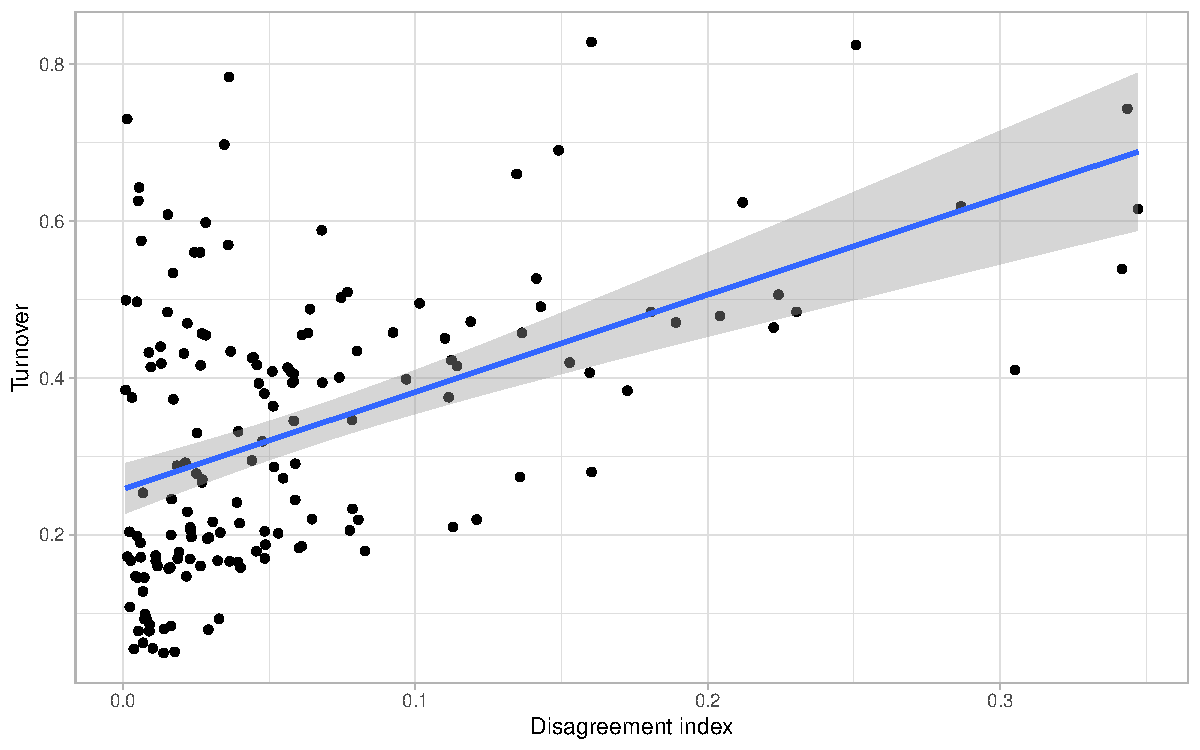
\includegraphics[width=0.8\textwidth]{figures/DI_turnover_scatter.pdf}
%     \end{center}
% %    \caption*{  \scriptsize Note: .\par} 
%     \vspace{0.0cm}
%     \label{fig: DI_turnover_scatter}
%     \caption*{  \scriptsize Note: Scatterplot of disagreement index and turnover for a sample without outliers.\par} 
% \end{figure}
